In recent years, Convolutional Neural Networks (CNN) \cite{Lecun89} have emerged as the new state-of-the-art learning framework for image recognition. Key to their success is the ability to learn from large quantities of labelled data the complex appearance of real-world objects. One of the most striking aspects of CNNs is their ability to learn generic visual features that generalise to many tasks. In particular, CNNs pre-trained on datasets such as ImageNet ILSVRC have been shown to obtain excellent results in recognition in other domains~\cite{Donahue13}, in object detection \cite{Girshick14}, in semantic segmentation \cite{Hariharan14}, in human pose estimation \cite{Toshev13}, and in many other tasks.

In this paper we look at how the power of CNNs can be leveraged in  \emph{weakly supervised detection} (WSD), which is the problem of learning object detectors using only image-level labels. The ability of learning from weak annotations is very important for two reasons: first, image understanding aims at learning an growing body of complex visual concepts (\eg hundred thousands object categories in ImageNet). Second, CNN training is data-hungry. Therefore, being able to learn complex concepts using only light supervision can reduce significantly the cost of data annotation in tasks such as image segmentation, image captioning, or object detection.

\begin{figure}
\begin{center}
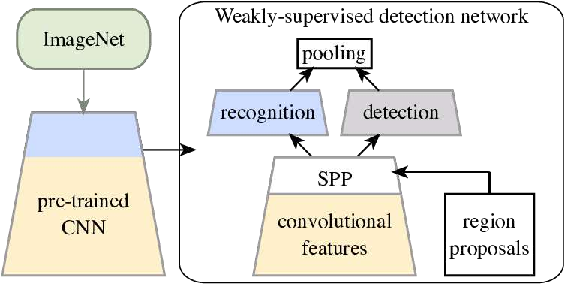
\includegraphics[width=\columnwidth]{splash} 
\end{center}
\caption{{\bf Weakly Supervised Deep Detection Network.} Our method starts from a CNN pre-trained for image classification on a large dataset, e.g. ImageNet. It then modifies to reason efficiently about regions, branching off a recognition and a detection data streams. The resulting architecture can be fine-tuned on a target dataset to achieve state-of-the-art weakly supervised object detection using only image-level annotations.}
\label{f:splash}
\end{figure}

We are motivated in our research by the hypothesis that, since pre-trained CNNs generalise so well to a large number of tasks, they should contain meaningful representations of the data. For example, there exists evidence that CNNs trained for image classification learn proxies to objects and objects parts~\cite{Zhou15}. Remarkably, these concepts are acquired implicitly, without ever providing the network with information about the \emph{location} of such structures in images. Hence, CNNs trained for image classification may already contain implicitly most of the information required to perform object detection.

We are not the first to address the problem of WSD with CNNs. The method of Wang~\etal~\cite{Wang14a}, for example, uses a pre-trained CNN to describe image regions and then learn object categories as corresponding visual topics. While this method is currently state-of-the-art in weakly supervised object detection, it comprises several components beyond the CNN and requires signifiant tuning. 

In this paper we contribute a novel {\em end-to-end} method for weakly supervised object detection using pre-trained CNNs which we call a \emph{weakly supervised deep detection network} (WSDDN) (\cref{f:splash}). Our method (\cref{s:method}) starts from an existing network, such as AlexNet pre-trained on ImageNet data, and extends it to reason explicitly and efficiently about image regions $R$. In order to do so, given an image $\bx$, the first step is to efficiently extract region-level descriptors $\phi(\bx;R)$ by inserting a spatial pyramid pooling layer on top of the convolutional layers of the CNN~\cite{He14,Girshick15}. Next,  the network is branched to extract \emph{two data streams} from the pooled region-level features. The first stream associates a class score $\phi^c(\bx;R)$ to each region individually, performing \emph{recognition}.  The second stream, instead, \emph{compares} regions by computing a probability distribution $\phi^d(\bx;R)$ over them; the latter represents the belief that, among all the candidate regions in the image,  $R$ is the one that contains the most salient image structure, and is therefore a proxy to \emph{detection}. The recognition and detection scores computed for all the image regions are finally aggregated in order to predict the class of the image as a whole, which is then used to inject image-level supervision in learning.

It is interesting to compare our method to the most common weakly supervised object detection technique, namely multiple instance learning (MIL)~\cite{Dietterich97}. MIL alternates between selecting which regions in images look like  the object of interest and estimating an appearance model of the object using the selected regions. Hence, MIL uses the appearance model itself to perform region selection. Our technique differs from MIL in a fundamental way as regions are selected by a dedicated \emph{parallel detection branch} in the network, which is independent of the recognition branch. In this manner, our approach helps avoiding one of the pitfalls of MIL, namely the tendency of the method to get stuck in local optima. 

Our two-stream CNN is also weakly related to the recent work of Lin~\etal~\cite{Lin15}. They propose a ``bilinear'' architecture where the output of two parallel network streams are combined by taking the outer product of feature vectors at corresponding spatial locations. The authors state that this construction is inspired by the ventral and dorsal streams of the human visual system, one focusing on recognition and the other one on localisation. While our architecture contains two such streams, the similarity is only superficial. A key difference is that in Lin~\etal the two streams are perfectly symmetric, and therefore there is no reason to believe that one should perform classification and the other detection; in our scheme, instead, the detection branch is explicitly designed to compare regions, breaking the symmetry. Note also that Lin~\etal~\cite{Lin15} do not perform WSD nor evaluate object detection performance.

Once the modifications have been applied, the network is ready to be fine-tuned on a target dataset, using only image-level labels, region proposals and back-propagation. In \cref{s:experiments} we show that, when fine-tuned on the PASCAL VOC training set, this architecture achieves state-of-the-art weakly supervised object detection on the PASCAL data, achieving superior results to the current state-of-the-art~\cite{Wang14a} but \emph{using only CNN machinery}. Since the system can be trained end-to-end using standard CNN packages, it is also as efficient as the recent fully-supervised Fast R-CNN detector of Girshick~\etal~\cite{Girshick15}, both in training and in testing. Finally, as a byproduct of our construction we also obtain a powerful image classifier that \emph{performs better than standard fine-tuning techniques} on the target data. Our findings are summarised in~\cref{s:conclusions}.
